% 1986 年广东卷文史类第 6 题：固定源题面三棱锥图（仅 S/A/B/C）
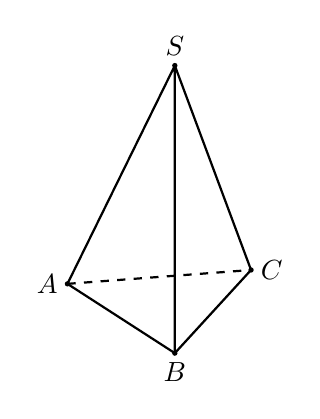
\begin{tikzpicture}[scale=0.88,>=stealth]
  \coordinate (A) at (0,0);
  \coordinate (B) at (1.55,-1.0);
  \coordinate (C) at (2.65,0.2);
  \coordinate (S) at (1.55,3.15);

  \draw[thick] (A)--(B)--(C);
  \draw[dashed,thick] (A)--(C);
  \draw[thick] (S)--(A) (S)--(B) (S)--(C);
  \fill (A) circle (1.1pt) node[left] {$A$};
  \fill (B) circle (1.1pt) node[below] {$B$};
  \fill (C) circle (1.1pt) node[right] {$C$};
  \fill (S) circle (1.1pt) node[above] {$S$};
\end{tikzpicture}
